% CanConnect Technical Documentation
% A comprehensive documentation for the CanConnect healthcare platform

\documentclass[12pt,a4paper]{report}
\usepackage[utf8]{inputenc}
\usepackage[T1]{fontenc}
\usepackage{lmodern}
\usepackage{microtype}
\usepackage{graphicx}
\usepackage{hyperref}
\usepackage{listings}
\usepackage{xcolor}
\usepackage{amsmath}
\usepackage{amssymb}
\usepackage{booktabs}
\usepackage{tabularx}
\usepackage{tikz}
\usepackage{float}
\usepackage{fancyhdr}
\usepackage{tocloft}
\usepackage{titlesec}
\usepackage{appendix}

% Define colors
\definecolor{medical-blue}{RGB}{42, 92, 130}
\definecolor{accent-teal}{RGB}{78, 205, 196}
\definecolor{code-background}{RGB}{248, 248, 248}
\definecolor{code-string}{RGB}{42, 161, 152}
\definecolor{code-comment}{RGB}{88, 110, 117}
\definecolor{code-keyword}{RGB}{203, 75, 22}

% Configure hyperref
\hypersetup{
    colorlinks=true,
    linkcolor=medical-blue,
    filecolor=medical-blue,
    urlcolor=accent-teal,
    citecolor=medical-blue
}

% Configure listings
\lstset{
    backgroundcolor=\color{code-background},
    basicstyle=\footnotesize\ttfamily,
    breakatwhitespace=false,
    breaklines=true,
    captionpos=b,
    commentstyle=\color{code-comment}\itshape,
    extendedchars=true,
    frame=single,
    keepspaces=true,
    keywordstyle=\color{code-keyword}\bfseries,
    language=JavaScript,
    numbers=left,
    numbersep=5pt,
    numberstyle=\tiny\color{code-comment},
    rulecolor=\color{black},
    showspaces=false,
    showstringspaces=false,
    showtabs=false,
    stepnumber=1,
    stringstyle=\color{code-string},
    tabsize=2,
    title=\lstname
}

% Configure page headers and footers
\pagestyle{fancy}
\fancyhf{}
\fancyhead[L]{CanConnect Technical Documentation}
\fancyhead[R]{\thepage}
\renewcommand{\headrulewidth}{0.4pt}
\renewcommand{\footrulewidth}{0pt}

% Title page formatting
\title{
    \vspace{-1cm}
    \includegraphics[width=0.8\textwidth]{logo.png}\\
    \Huge\textbf{CanConnect}\\
    \Large Technical Documentation\\
    \vspace{0.5cm}
    \large A Comprehensive Healthcare Platform for Cancer Care Coordination
}
\author{Development Team}
\date{\today}

\begin{document}

\maketitle
\tableofcontents
\newpage

\chapter{Introduction}

\section{Project Overview}
CanConnect is a comprehensive healthcare platform designed to facilitate communication and coordination between cancer patients, doctors, patient navigators, and caregivers. The system aims to streamline the cancer care journey by connecting all stakeholders in the treatment process, providing specialized interfaces for different user roles, and facilitating efficient patient care management.

\section{Scope and Objectives}
The primary objective of CanConnect is to improve the overall cancer patient experience by:
\begin{itemize}
    \item Facilitating seamless communication between patients and healthcare providers
    \item Providing a consolidated platform for managing medical records and treatment plans
    \item Streamlining the coordination of care services through patient navigators
    \item Supporting caregivers with tools and resources for effective patient assistance
    \item Creating a comprehensive resource center for patients to access educational materials
    \item Enabling healthcare providers to efficiently manage patient information and treatment plans
\end{itemize}

\section{Document Purpose}
This technical documentation provides detailed information about the CanConnect platform's architecture, components, implementation, and deployment. It serves as a comprehensive reference for developers, system administrators, and other technical stakeholders involved in the development, maintenance, and extension of the platform.

\chapter{System Architecture}

\section{High-Level Architecture}
CanConnect follows a traditional web application architecture with a client-server model:

\begin{figure}[H]
\centering
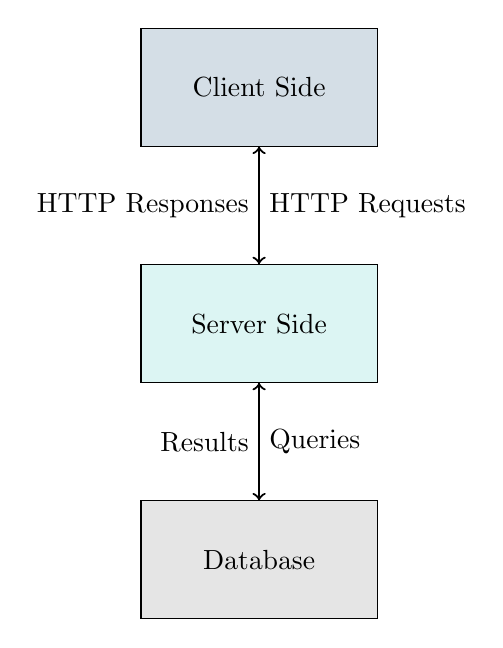
\begin{tikzpicture}
    \node[draw, rectangle, minimum width=3cm, minimum height=1.5cm, fill=medical-blue!20] (client) at (0,0) {Client Side};
    \node[draw, rectangle, minimum width=3cm, minimum height=1.5cm, fill=accent-teal!20] (server) at (0,-3) {Server Side};
    \node[draw, rectangle, minimum width=3cm, minimum height=1.5cm, fill=gray!20] (db) at (0,-6) {Database};
    
    \draw[->, thick] (client) -- node[right] {HTTP Requests} (server);
    \draw[->, thick] (server) -- node[left] {HTTP Responses} (client);
    \draw[->, thick] (server) -- node[right] {Queries} (db);
    \draw[->, thick] (db) -- node[left] {Results} (server);
\end{tikzpicture}
\caption{High-level architecture of CanConnect}
\end{figure}

\section{Technology Stack}
\begin{table}[H]
\centering
\begin{tabularx}{\textwidth}{lX}
\toprule
\textbf{Component} & \textbf{Technology} \\
\midrule
Backend Framework & Node.js with Express.js \\
Frontend & EJS templating engine with Bootstrap 5 \\
Database & MongoDB with Mongoose ODM \\
Authentication & Passport.js with local strategy \\
Session Management & express-session with connect-mongo \\
Data Visualization & Chart.js \\
UI Components & Bootstrap 5, Font Awesome \\
Development Tools & nodemon (development server) \\
\bottomrule
\end{tabularx}
\caption{Technology stack overview}
\end{table}

\section{System Components}
The system is divided into the following major components:

\subsection{Authentication System}
Handles user registration, login, and session management using Passport.js for authentication and authorization. The system supports four user roles: Patient, Doctor, Patient Navigator, and Caregiver.

\subsection{User Management}
Manages user profiles, permissions, and role-based access control. User data is stored in MongoDB with specific fields based on user roles.

\subsection{Patient Portal}
Provides patients with access to their medical records, appointment schedules, treatment plans, and educational resources. Includes features for feedback submission and communication with healthcare providers.

\subsection{Doctor Interface}
Enables physicians to manage patient appointments, review medical records, create treatment plans, and monitor patient progress. Includes a dashboard with key metrics and patient statistics.

\subsection{Patient Navigator Module}
Facilitates the coordination of patient care services, resource allocation, and communication between patients and healthcare providers.

\subsection{Caregiver Access}
Provides caregivers with limited access to patient information, appointment schedules, and educational resources to support patient care.

\subsection{Resource Center}
A centralized repository of educational materials, support resources, and guidelines for patients, caregivers, and healthcare providers.

\chapter{Database Design}

\section{Database Model}
CanConnect uses MongoDB, a NoSQL document database, for data storage. Mongoose is used as an ODM (Object Document Mapper) to structure the data and enforce data validation.

\section{Schema Definitions}

\subsection{User Schema}
The primary user schema stores authentication information and basic user details:

\begin{lstlisting}[language=JavaScript]
const UserSchema = new mongoose.Schema({
  fullName: {
    type: String,
    required: true,
  },
  email: {
    type: String,
    required: true,
    unique: true,
  },
  age: {
    type: Number,
    required: true,
  },
  phone: {
    type: String,
    required: true,
  },
  sex: {
    type: String,
    enum: ["Male", "Female"],
    required: true,
  },
  address: {
    type: String,
    required: true,
  },
  userType: {
    type: String,
    enum: ["Patient", "Patient-Navigator", "Caregiver", "Doctor"],
    required: true,
  },
  // Doctor-specific fields
  specialization: {
    type: String,
    required: function() {
      return this.userType === "Doctor";
    }
  },
  experience: {
    type: Number,
    required: function() {
      return this.userType === "Doctor";
    }
  },
  hospital: {
    type: String,
    required: function() {
      return this.userType === "Doctor";
    }
  },
  profileImage: {
    type: String,
    default: "/images/default-doctor.png"
  },
  licenseNumber: {
    type: String,
    required: function() {
      return this.userType === "Doctor";
    }
  }
});
\end{lstlisting}

\subsection{Patient Schema}
For storing detailed patient information, the system uses an extended schema that follows the HL7 FHIR standard for healthcare interoperability:

\begin{lstlisting}[language=JavaScript]
const PatientSchema = new mongoose.Schema({
  meta: {
    profile: {
      type: [String],
      default: ['http://hl7.org/fhir/us/mcode/StructureDefinition/mcode-cancer-patient'],
      required: true
    }
  },
  identifier: {
    type: [IdentifierSchema],
    validate: arrayValidator(1, 5)
  },
  name: {
    type: [HumanNameSchema],
    validate: arrayValidator(1, 3)
  },
  gender: {
    type: String,
    enum: ['male', 'female', 'other', 'unknown'],
    required: true
  },
  birthDate: {
    type: Date,
    required: true
  },
  deceasedBoolean: Boolean,
  deceasedDateTime: Date,
  address: [AddressSchema],
  telecom: [ContactPointSchema],
  extension: {
    type: [ExtensionSchema],
    validate: {
      validator: function(extensions) {
        const requiredUrls = [
          'http://hl7.org/fhir/us/core/StructureDefinition/us-core-race',
          'http://hl7.org/fhir/us/core/StructureDefinition/us-core-ethnicity',
          'http://hl7.org/fhir/us/core/StructureDefinition/us-core-birthsex',
          'http://hl7.org/fhir/us/core/StructureDefinition/us-core-genderIdentity'
        ];
        return requiredUrls.every(url => 
          extensions.some(ext => ext.url === url)
        );
      },
      message: 'Missing required extensions'
    }
  }
});
\end{lstlisting}

\section{Database Relationships}
The application uses MongoDB's reference model to establish relationships between collections. For example:

\begin{itemize}
    \item A doctor can have many patients
    \item A patient can have one primary doctor
    \item A patient navigator can manage multiple patients
    \item A patient can have multiple appointments
    \item A caregiver can be associated with one or more patients
\end{itemize}

\section{Data Validation and Security}
The application implements several layers of data validation and security:

\begin{itemize}
    \item Schema-level validation using Mongoose validators
    \item Custom validators for complex validation rules
    \item Encryption of sensitive patient information
    \item Role-based access control for data access
\end{itemize}

\chapter{Application Structure}

\section{Directory Organization}
The application follows a modular structure to organize code and assets:

\begin{lstlisting}
CanConnect/
├── models/              # Database models
├── routes/              # Route handlers
├── views/              
│   ├── pages/          # Page templates
│   │   ├── auth/       # Authentication pages
│   │   ├── doctor/     # Doctor interface
│   │   ├── patient/    # Patient interface
│   │   └── navigator/  # Navigator interface
│   ├── layouts/        # Layout templates
│   └── partials/       # Reusable components
├── public/             # Static files
├── middlewares/        # Custom middleware
├── app.js              # Application entry point
└── package.json        # Dependencies
\end{lstlisting}

\section{Route Structure}
The application routes are organized by user role to maintain clear separation of concerns:

\subsection{Authentication Routes}
Handles user registration, login, logout, and password management:

\begin{lstlisting}[language=JavaScript]
// Example of authentication routes
router.get("/login", (req, res) => {
  res.render("pages/auth/login");
});

router.post("/login", passport.authenticate("local", {
  failureRedirect: "/login",
  failureFlash: true
}), (req, res) => {
  const userType = req.user.userType.toLowerCase();
  res.redirect(`/${userType}/dashboard`);
});

router.get("/logout", (req, res) => {
  req.logout();
  res.redirect("/login");
});
\end{lstlisting}

\subsection{Doctor Routes}
Manages doctor-specific functionality:

\begin{lstlisting}[language=JavaScript]
// Doctor dashboard route
router.get("/dashboard", isLoggedIn, (req, res) => {
  if (req.user.userType !== "Doctor") {
    return res.redirect(`/${req.user.userType.toLowerCase()}/dashboard`);
  }

  // Mock data for demonstration - replace with actual database queries
  const dashboardData = {
    todayAppointments: 8,
    pendingRequests: 5,
    feedbackCount: 12,
    highRiskPatients: 4,
    recentAppointments: [
      {
        id: 1,
        patientName: "John Doe",
        time: "10:30 AM",
        status: "Completed"
      },
      {
        id: 2,
        patientName: "Jane Smith",
        time: "11:45 AM",
        status: "Pending"
      },
      {
        id: 3,
        patientName: "Robert Johnson",
        time: "2:15 PM",
        status: "Pending"
      }
    ],
    patientStats: {
      newPatients: 15,
      regularPatients: 45,
      highRisk: 8
    }
  };

  res.render("pages/doctor/dashboard.ejs", { 
    title: "Dashboard",
    page: "dashboard",
    doctor: {
      fullName: req.user.fullName,
      specialization: req.user.specialization
    },
    ...dashboardData
  });
});
\end{lstlisting}

\subsection{Patient Routes}
Manages patient-specific functionality:

\begin{lstlisting}[language=JavaScript]
// Patient dashboard route
router.get("/dashboard", isLoggedIn, (req, res) => {
  if (req.user.userType !== "Patient") {
    return res.redirect(`/${req.user.userType.toLowerCase()}/dashboard`);
  }
  const currentUser = {
    fullName: req.user.fullName,
    email: req.user.email,
    id: req.user.id,
  };
  res.render("pages/patient/dashboard.ejs", {
    currentUser: currentUser,
    activePage: "dashboard",
  });
});
\end{lstlisting}

\section{View Templates}
The application uses EJS (Embedded JavaScript) templating engine to render views. Templates are organized into layouts, pages, and partials:

\subsection{Layouts}
Layout templates define the overall structure of pages:

\begin{lstlisting}[language=HTML]
<!DOCTYPE html>
<html lang="en">
<head>
    <meta charset="UTF-8">
    <meta name="viewport" content="width=device-width, initial-scale=1.0">
    <title>CanConnect - Doctor <%= title %></title>
    <link href="https://cdn.jsdelivr.net/npm/bootstrap@5.3.0/dist/css/bootstrap.min.css" rel="stylesheet">
    <link href="https://cdnjs.cloudflare.com/ajax/libs/font-awesome/6.0.0/css/all.min.css" rel="stylesheet">
    <style>
        :root {
            --primary-blue: #2a5c82;
            --secondary-blue: #5c9baf;
            --accent-teal: #4ecdc4;
            --high-risk: #dc3545;
            --medium-risk: #ffc107;
            --low-risk: #28a745;
            --sidebar-width: 250px;
            --header-height: 60px;
        }
        /* Additional styles... */
    </style>
</head>
<body>
    <nav class="navbar medical-header">
        <!-- Header content -->
    </nav>

    <div class="d-flex">
        <!-- Sidebar Container -->
        <div class="sidebar-container" id="sidebar">
            <%- include('../partials/doctor-sidebar', { 
                doctor: doctor,
                page: page 
            }) %>
        </div>
        
        <!-- Main Content -->
        <div class="main-content flex-grow-1">
            <%- include('../' + content) %>
        </div>
    </div>

    <script src="https://cdn.jsdelivr.net/npm/bootstrap@5.3.0/dist/js/bootstrap.bundle.min.js"></script>
    <script>
        // JavaScript functionality
    </script>
</body>
</html>
\end{lstlisting}

\subsection{Page Templates}
Page templates contain the specific content for each route:

\begin{lstlisting}[language=HTML]
<!-- Doctor Dashboard Content -->
<div class="container-fluid">
  <div class="row mb-4">
    <div class="col-md-3">
      <div class="card card-medical">
        <div class="card-body">
          <h5 class="card-title">Today's Appointments</h5>
          <h2 class="text-primary"><%= todayAppointments %></h2>
          <p class="text-muted">Scheduled for today</p>
        </div>
      </div>
    </div>
    <!-- Additional dashboard cards -->
  </div>

  <div class="row">
    <div class="col-md-8">
      <div class="card card-medical">
        <div class="card-body">
          <h5 class="card-title">Recent Appointments</h5>
          <div class="table-responsive">
            <table class="table">
              <!-- Table content -->
            </table>
          </div>
        </div>
      </div>
    </div>
    <div class="col-md-4">
      <div class="card card-medical">
        <div class="card-body">
          <h5 class="card-title">Patient Statistics</h5>
          <canvas id="patientStatsChart"></canvas>
        </div>
      </div>
    </div>
  </div>
</div>

<script src="https://cdn.jsdelivr.net/npm/chart.js"></script>
<script>
  const ctx = document.getElementById('patientStatsChart').getContext('2d');
  new Chart(ctx, {
    type: 'doughnut',
    data: {
      labels: ['New Patients', 'Regular Patients', 'High-Risk'],
      datasets: [{
        data: [<%= patientStats.newPatients %>, <%= patientStats.regularPatients %>, <%= patientStats.highRisk %>],
        backgroundColor: ['#4ecdc4', '#2a5c82', '#dc3545']
      }]
    },
    options: {
      responsive: true,
      maintainAspectRatio: false
    }
  });
</script>
\end{lstlisting}

\chapter{Authentication and Security}

\section{Authentication Implementation}
CanConnect uses Passport.js for authentication, with a local strategy based on username and password:

\begin{lstlisting}[language=JavaScript]
// Configure Passport-Local Strategy
passport.use(new LocalStrategy(User.authenticate()));
passport.serializeUser(User.serializeUser());
passport.deserializeUser(User.deserializeUser());
\end{lstlisting}

\section{Session Management}
Sessions are managed using express-session with MongoDB as the session store:

\begin{lstlisting}[language=JavaScript]
// Configure session with improved persistence
app.use(
  session({
    secret: process.env.SESSION_SECRET || "our little secret",
    resave: false,
    saveUninitialized: false,
    cookie: {
      httpOnly: true,
      maxAge: 7 * 24 * 60 * 60 * 1000, // 7 days in milliseconds
      secure: process.env.NODE_ENV === "production", // secure in production only
    },
    store: MongoStore.create({
      mongoUrl: ATLASDB_URL,
      touchAfter: 24 * 3600, // time period in seconds to refresh session (1 day)
    }),
  })
);
\end{lstlisting}

\section{Role-Based Access Control}
The application implements role-based access control through middleware:

\begin{lstlisting}[language=JavaScript]
// Authentication middleware
const isLoggedIn = (req, res, next) => {
  if (req.isAuthenticated()) {
    return next();
  }
  res.redirect("/login");
};

// Role-specific middleware
const isDoctorUser = (req, res, next) => {
  if (req.user.userType === "Doctor") {
    return next();
  }
  res.redirect(`/${req.user.userType.toLowerCase()}/dashboard`);
};
\end{lstlisting}

\section{Security Considerations}
The application implements several security measures:

\begin{itemize}
    \item Password hashing using Passport-Local-Mongoose
    \item HTTP-only cookies for session management
    \item Secure cookies in production environment
    \item CSRF protection
    \item Input validation and sanitization
    \item Role-based access control
    \item MongoDB security best practices
\end{itemize}

\chapter{User Interfaces}

\section{Design System}
The application uses a consistent design system with predefined colors, typography, and components:

\begin{lstlisting}[language=CSS]
:root {
    --primary-blue: #2a5c82;
    --secondary-blue: #5c9baf;
    --accent-teal: #4ecdc4;
    --high-risk: #dc3545;
    --medium-risk: #ffc107;
    --low-risk: #28a745;
    --sidebar-width: 250px;
    --header-height: 60px;
}
\end{lstlisting}

\section{Responsive Design}
The application is designed to be responsive across various device sizes:

\begin{lstlisting}[language=CSS]
@media (max-width: 768px) {
    .sidebar-container {
        transform: translateX(-100%);
    }
    .sidebar-container.show {
        transform: translateX(0);
    }
    .main-content {
        margin-left: 0;
    }
}
\end{lstlisting}

\section{User Interface Components}
The application uses Bootstrap 5 for UI components, with custom styling to match the healthcare domain:

\begin{itemize}
    \item Navigation bar and sidebar for easy navigation
    \item Dashboard cards for key metrics
    \item Responsive tables for data display
    \item Charts and visualizations using Chart.js
    \item Forms with validation for data input
    \item Modal dialogs for confirmations and alerts
    \item Toast notifications for non-disruptive feedback
\end{itemize}

\chapter{Data Visualization}

\section{Chart.js Implementation}
The application uses Chart.js for data visualization:

\begin{lstlisting}[language=JavaScript]
const ctx = document.getElementById('patientStatsChart').getContext('2d');
new Chart(ctx, {
  type: 'doughnut',
  data: {
    labels: ['New Patients', 'Regular Patients', 'High-Risk'],
    datasets: [{
      data: [<%= patientStats.newPatients %>, <%= patientStats.regularPatients %>, <%= patientStats.highRisk %>],
      backgroundColor: ['#4ecdc4', '#2a5c82', '#dc3545']
    }]
  },
  options: {
    responsive: true,
    maintainAspectRatio: false
  }
});
\end{lstlisting}

\section{Dashboard Metrics}
The doctor dashboard displays key metrics for quick assessment:

\begin{itemize}
    \item Today's appointments
    \item Pending requests
    \item Patient feedback
    \item High-risk patients
    \item Patient statistics (new, regular, high-risk)
\end{itemize}

\chapter{Deployment and Environment Configuration}

\section{Environment Variables}
The application uses environment variables for configuration:

\begin{lstlisting}
PORT=3000
ATLASDB_URL=mongodb://localhost:27017/cancer_navigation
SESSION_SECRET=your_session_secret
\end{lstlisting}

\section{Development Environment}
For development, the application uses Nodemon for automatic server restarts:

\begin{lstlisting}[language=JSON]
"scripts": {
  "start": "node app.js",
  "dev": "nodemon app.js",
  "test": "echo \"Error: no test specified\" && exit 1"
}
\end{lstlisting}

\section{Production Deployment}
For production deployment, the application can be deployed to cloud platforms like:

\begin{itemize}
    \item Heroku
    \item AWS Elastic Beanstalk
    \item Google Cloud App Engine
    \item DigitalOcean App Platform
\end{itemize}

\section{Database Setup}
MongoDB Atlas is recommended for production database hosting, with appropriate security configurations:

\begin{itemize}
    \item IP whitelisting
    \item Strong authentication credentials
    \item Network encryption
    \item Database backup and recovery
\end{itemize}

\chapter{Testing Strategy}

\section{Unit Testing}
Unit tests focus on individual components and functions:

\begin{itemize}
    \item Model validation
    \item Authentication logic
    \item Business logic functions
    \item Utility functions
\end{itemize}

\section{Integration Testing}
Integration tests verify the interaction between components:

\begin{itemize}
    \item API endpoint testing
    \item Database operations
    \item Authentication flow
    \item Session management
\end{itemize}

\section{End-to-End Testing}
End-to-end tests simulate user interactions:

\begin{itemize}
    \item User registration and login
    \item Dashboard navigation
    \item Form submissions
    \item Data visualization
\end{itemize}

\chapter{Performance Optimization}

\section{Server-Side Optimization}
Server-side optimization strategies include:

\begin{itemize}
    \item Database query optimization
    \item Caching frequently accessed data
    \item Pagination for large data sets
    \item Efficient session management
\end{itemize}

\section{Client-Side Optimization}
Client-side optimization strategies include:

\begin{itemize}
    \item Minimizing CSS and JavaScript
    \item Implementing lazy loading for images
    \item Using CDN for static assets
    \item Optimizing chart rendering
\end{itemize}

\chapter{Future Enhancements}

\section{Planned Features}
Future enhancements for the platform include:

\begin{itemize}
    \item Mobile application development
    \item Integration with hospital management systems
    \item Advanced analytics and reporting
    \item Telemedicine features
    \item AI-powered recommendations
    \item Integration with wearable devices for patient monitoring
    \item Advanced notification system
    \item Enhanced security features
    \item Multi-language support
\end{itemize}

\section{Architectural Improvements}
Potential architectural improvements include:

\begin{itemize}
    \item Microservices architecture
    \item GraphQL API implementation
    \item WebSocket integration for real-time updates
    \item Docker containerization
    \item Kubernetes orchestration
    \item Serverless computing for specific functions
\end{itemize}

\chapter{Conclusion}

\section{Summary}
CanConnect represents a comprehensive solution for cancer care coordination, bringing together patients, doctors, navigators, and caregivers on a single platform. The application's architecture and implementation provide a solid foundation for current functionality while allowing for future expansion and enhancement.

\section{Recommendations}
Based on the current implementation, the following recommendations are made:

\begin{itemize}
    \item Implement comprehensive automated testing
    \item Enhance data security measures for sensitive patient information
    \item Optimize database queries for improved performance
    \item Develop a mobile application to complement the web platform
    \item Implement real-time notification features
    \item Explore integration with electronic health record (EHR) systems
\end{itemize}

\appendix
\chapter{API Documentation}

\section{Authentication Endpoints}
\begin{itemize}
    \item POST /login - User authentication
    \item GET /logout - User logout
    \item POST /register - User registration
    \item POST /reset-password - Password reset
\end{itemize}

\section{Doctor Endpoints}
\begin{itemize}
    \item GET /doctor/dashboard - Doctor dashboard
    \item GET /doctor/appointment-management - Appointment management
    \item GET /doctor/patient-info - Patient information
    \item GET /doctor/progress-reports - Progress reports
    \item GET /doctor/feedback-management - Feedback management
    \item GET /doctor/resources - Resources access
\end{itemize}

\section{Patient Endpoints}
\begin{itemize}
    \item GET /patient/dashboard - Patient dashboard
    \item GET /patient/appointments - Appointment management
    \item GET /patient/care-plan - Care plan access
    \item GET /patient/initial-registration - Initial registration
    \item GET /patient/feedback - Feedback submission
    \item GET /patient/patient-profile - Patient profile
    \item GET /patient/reports - Medical reports
    \item GET /patient/cancer-details - Cancer details
\end{itemize}

\chapter{Database Schema Reference}

\section{User Schema}
Detailed documentation of the User schema fields, validation rules, and relationships.

\section{Patient Schema}
Detailed documentation of the Patient schema fields, validation rules, and relationships.

\section{Appointment Schema}
Detailed documentation of the Appointment schema fields, validation rules, and relationships.

\section{Medical Record Schema}
Detailed documentation of the Medical Record schema fields, validation rules, and relationships.

\chapter{Development Guidelines}

\section{Coding Standards}
Documentation of coding standards for JavaScript, CSS, and HTML.

\section{Git Workflow}
Guidelines for Git branching, commit messages, and pull request processes.

\section{Documentation Requirements}
Guidelines for code documentation, API documentation, and user documentation.

\bibliographystyle{plain}
\bibliography{references}

\end{document} 